\chapter{System Overview and Problem Formulation}
\label{chap:system_overview}
\section{System Overview}
The system consists of a six-degree-of-freedom manipulator, a polishing spindle, a wrist six-axis force/torque sensor, a CAD or reconstructed workpiece model, one or more RGB or RGB-D cameras, and a rigid fixture. The framework contains four high-level components: a geometric full-coverage planner, an RL process optimizer, a force-aware IL local planner, and a feature-masking module. All trajectories are executed by a deterministic low-level admittance controller and filtered by an independent safety supervisor.

\begin{figure}[t]
    \centering
    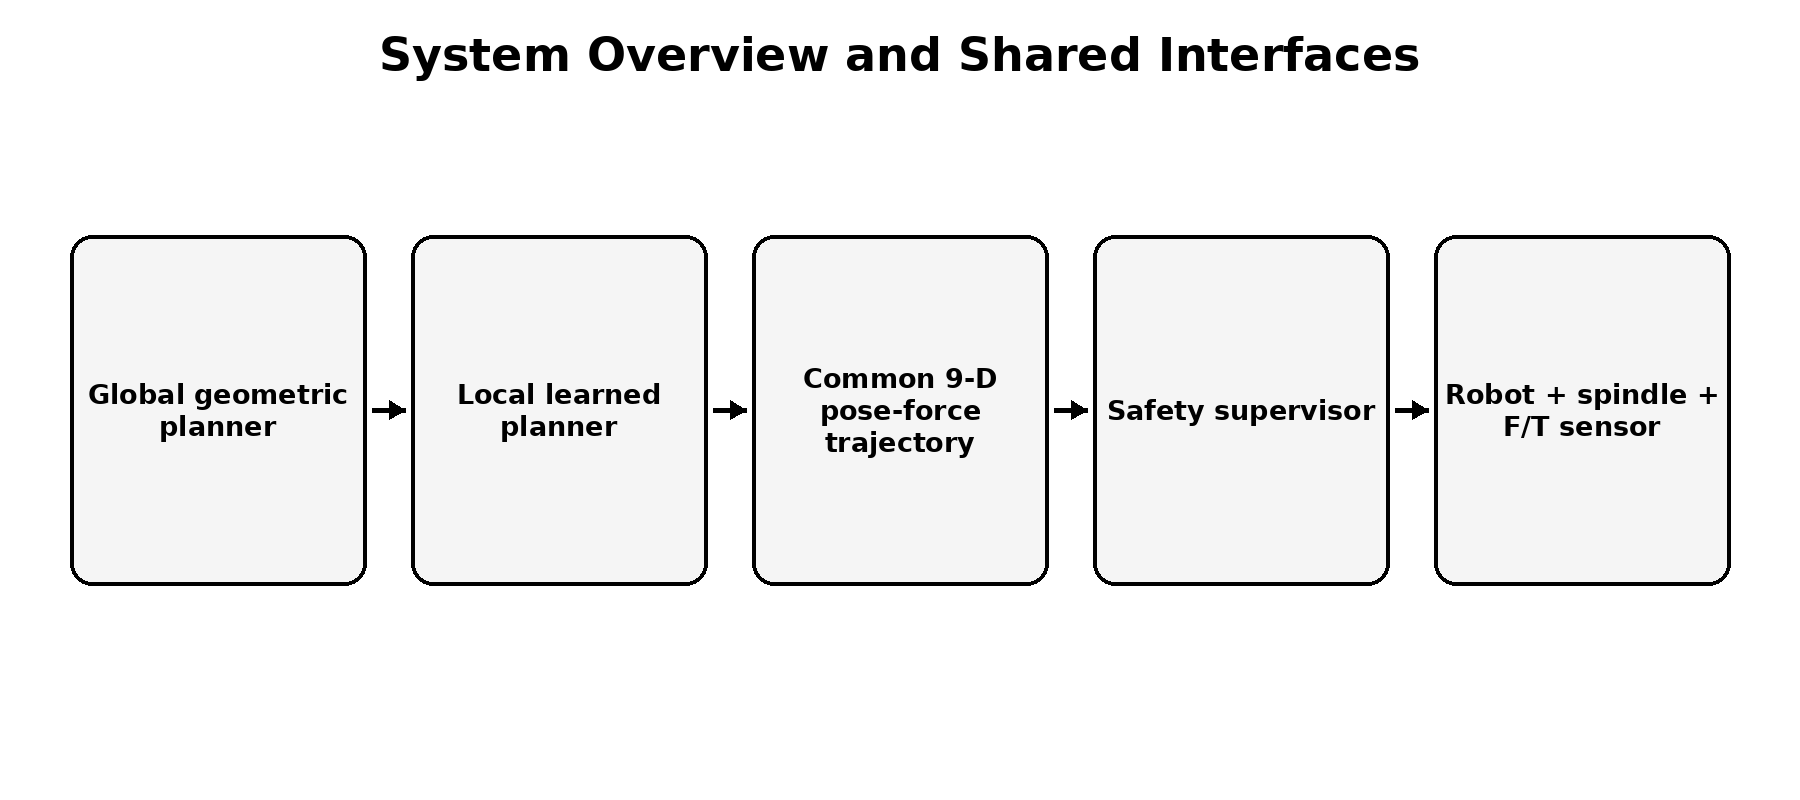
\includegraphics[width=0.98\textwidth]{./2.SystemOverview/figs/system_overview.png}
    \caption{System modules and shared interfaces.}
    \label{fig:system_overview}
\end{figure}

\section{Task Decomposition}
Let $\mathcal{S}$ denote the workpiece surface and $\Omega\subset\mathcal{S}$ the target finishing region. The complete task is partitioned into a global geometric region $\Omega_g$ and a set of local difficult regions $\{\Omega_{\ell}^{i}\}_{i=1}^{N_\ell}$:
\begin{equation}
\Omega = \Omega_g \cup \bigcup_{i=1}^{N_\ell}\Omega_{\ell}^{i}, \qquad \Omega_g \cap \Omega_{\ell}^{i}=\varnothing.
\end{equation}
The global region contains broad, continuous, and reliably modeled surfaces. Local regions contain sharp boundaries, small reflective hardware, narrow clearance, incomplete reconstruction, or contact behavior that requires configuration-dependent expert adjustment. Initial experiments may use manual region annotation; automatic assignment based on reconstruction confidence, curvature, clearance, and planner feasibility is reserved for future work.

\section{Common Pose--Force Trajectory}
Both the geometric planner and the IL policy generate a dense sequence of 9-D waypoints:
\begin{equation}
\mathbf{a}_k = [x_k,y_k,z_k,\omega_{x,k},\omega_{y,k},\omega_{z,k},F_{x,k},F_{y,k},F_{z,k}]^{\top}.
\end{equation}
The first six variables define the desired end-effector pose, with orientation represented as a rotation vector. The final three variables define the desired Cartesian force. The global planner derives pose from CAD geometry and uses a prescribed force profile. The local IL policy predicts the complete pose--force action chunk from sensory observations.

\section{Admittance-Controlled Execution}
The high-level trajectory does not directly produce joint torques. A Cartesian admittance controller computes a compliant pose correction from the desired and measured wrench:
\begin{equation}
\mathbf{M}_d\Delta\ddot{\mathbf{x}}+\mathbf{D}_d\Delta\dot{\mathbf{x}}+\mathbf{K}_d\Delta\mathbf{x}=\mathbf{F}_d-\mathbf{F}_m.
\end{equation}
The controller maintains high-rate contact stability, while the high-level modules determine the global path, local strategy, and desired sliding speed. This separation is essential for fair evaluation: improvements caused by deterministic force control must not be incorrectly attributed to a learning policy.

\section{Safety Supervisor}
Hard limits are imposed on workspace, joint range, self-collision, workpiece collision, force, torque, velocity, acceleration, spindle state, and cumulative dwell. The supervisor can clip a velocity scale, reject a predicted waypoint, pause the spindle, or command a controlled retraction. Learning policies are therefore optimized within a bounded execution envelope.

\section{Demonstration Object: Guitar}
A guitar is used as the principal validation object because it combines broad coated surfaces and local difficult features in one product. The body top, back, and side are suitable for CAD-based coverage. The body edge, cutaway, neck joint, frets, pickup covers, bridge, and other metal hardware expose narrow, reflective, and contact-sensitive regions. The object is also compact enough for a UR10e-class robot and supports both manufacturing-oriented body finishing and repair-oriented local reconditioning.
